\documentclass[a4paper, 11pt]{article}
\usepackage[polish]{babel}
\usepackage[T1]{fontenc}
\usepackage{hyperref}
\usepackage{array}
\usepackage{amssymb}
\usepackage{amsmath}
\usepackage{changepage}
\usepackage{multicol}
\usepackage[margin=1in]{geometry}
\hypersetup{
    colorlinks,
    citecolor=black,
    filecolor=black,
    linkcolor=black,
    urlcolor=black
}
\usepackage{graphicx}

\usepackage{tikz}
\usetikzlibrary{fit,arrows,matrix,positioning, calc, shapes.gates.logic.IEC, shapes.gates.logic.US}
\usetikzlibrary {arrows.meta}
\tikzstyle{branch}=[fill,shape=circle,minimum size=3pt,inner sep=0pt]


\title{%
        \vspace{-1cm}
       \large Sprawozdanie Laboratorium Fizyka dla informatyków \\
       \huge Wyznaczanie współczynnika rozszerzalności liniowej ciał stałych.}

\author{Stanisław Fiedler 160250}
\date{LAB 2, 12 listopada 2024}

\begin{document}
\begin{table}
	\begin{adjustwidth}{-0.25\textwidth}{-0.25\textwidth}
		\begin{center}
			\begin{tabular}{|l|l|l|l|l|}
				\hline
				Nr Ćwiczenia 103                                             & Data wykonania 12.11.2024                 & Wydział WIiT & Semestr 3 & Grupa LAB L1 \\
				\hline
				\multicolumn{2}{|l|}{ Prowadzący: mgr inż. Taras Zhezhera  } & \multicolumn{2}{|l|}{ Stanisław Fiedler } & Ocena:                                  \\
				\hline
			\end{tabular}
		\end{center}
	\end{adjustwidth}
\end{table}

\maketitle
\tableofcontents

\section{Wstęp teoretyczny}\label{sec:wstep} % (fold)
Zmianie temperatury ciała towarzyszy na ogół zmiana jego wymiarów linowych,
a więc także zmiana jego objętości.
Przyrost temperatury $dT$ ciała, którego długość całkowita wynosi l,
powoduje przyrost długości $dl$ określony wzorem:
\begin{equation}\label{eq:alpha1}
	dl = \alpha l\,dT
\end{equation}
Współczynnik $\alpha$ nazywamy współczynnikiem rozszerzalności liniowej.
W zakresie niewielkich zmian temperatury możemy przyjąć, że współczynnik $\alpha$ jest stały,
a długość wzrasta wprost proporcjonalnie do temperatury.
W tym przypadku odpowiednikiem wzoru \eqref{eq:alpha1} jest wzór:
\begin{equation}\label{eq:alpha2}
	l - l_0 = \alpha_{sr}l_o \Delta T
\end{equation}
\begin{equation}\label{eq:alpha3}
	\alpha_{sr} = \frac{l - l_0}{l_0 \Delta T}
\end{equation}

Przyczyna rozszerzalności cieplnej leży w strukturze mikroskopowej ciał.
Ciała zbudowane są z atomów tworzących sieć krystaliczną.
Dostarczona energia cieplna powoduje drgania atomów wokół położeń równowagi.
Amplituda tych drgań rośnie wraz z temperaturą.
Wraz ze wzrostem amplitudy drgań roście średnia odległość między atomami co obserwujemy jako rozszerzalność cieplna.

% section wstep (end)

\section{Wyniki pomiarów}\label{sec:wyniki_pomiarow} % (fold)

\begin{center}
	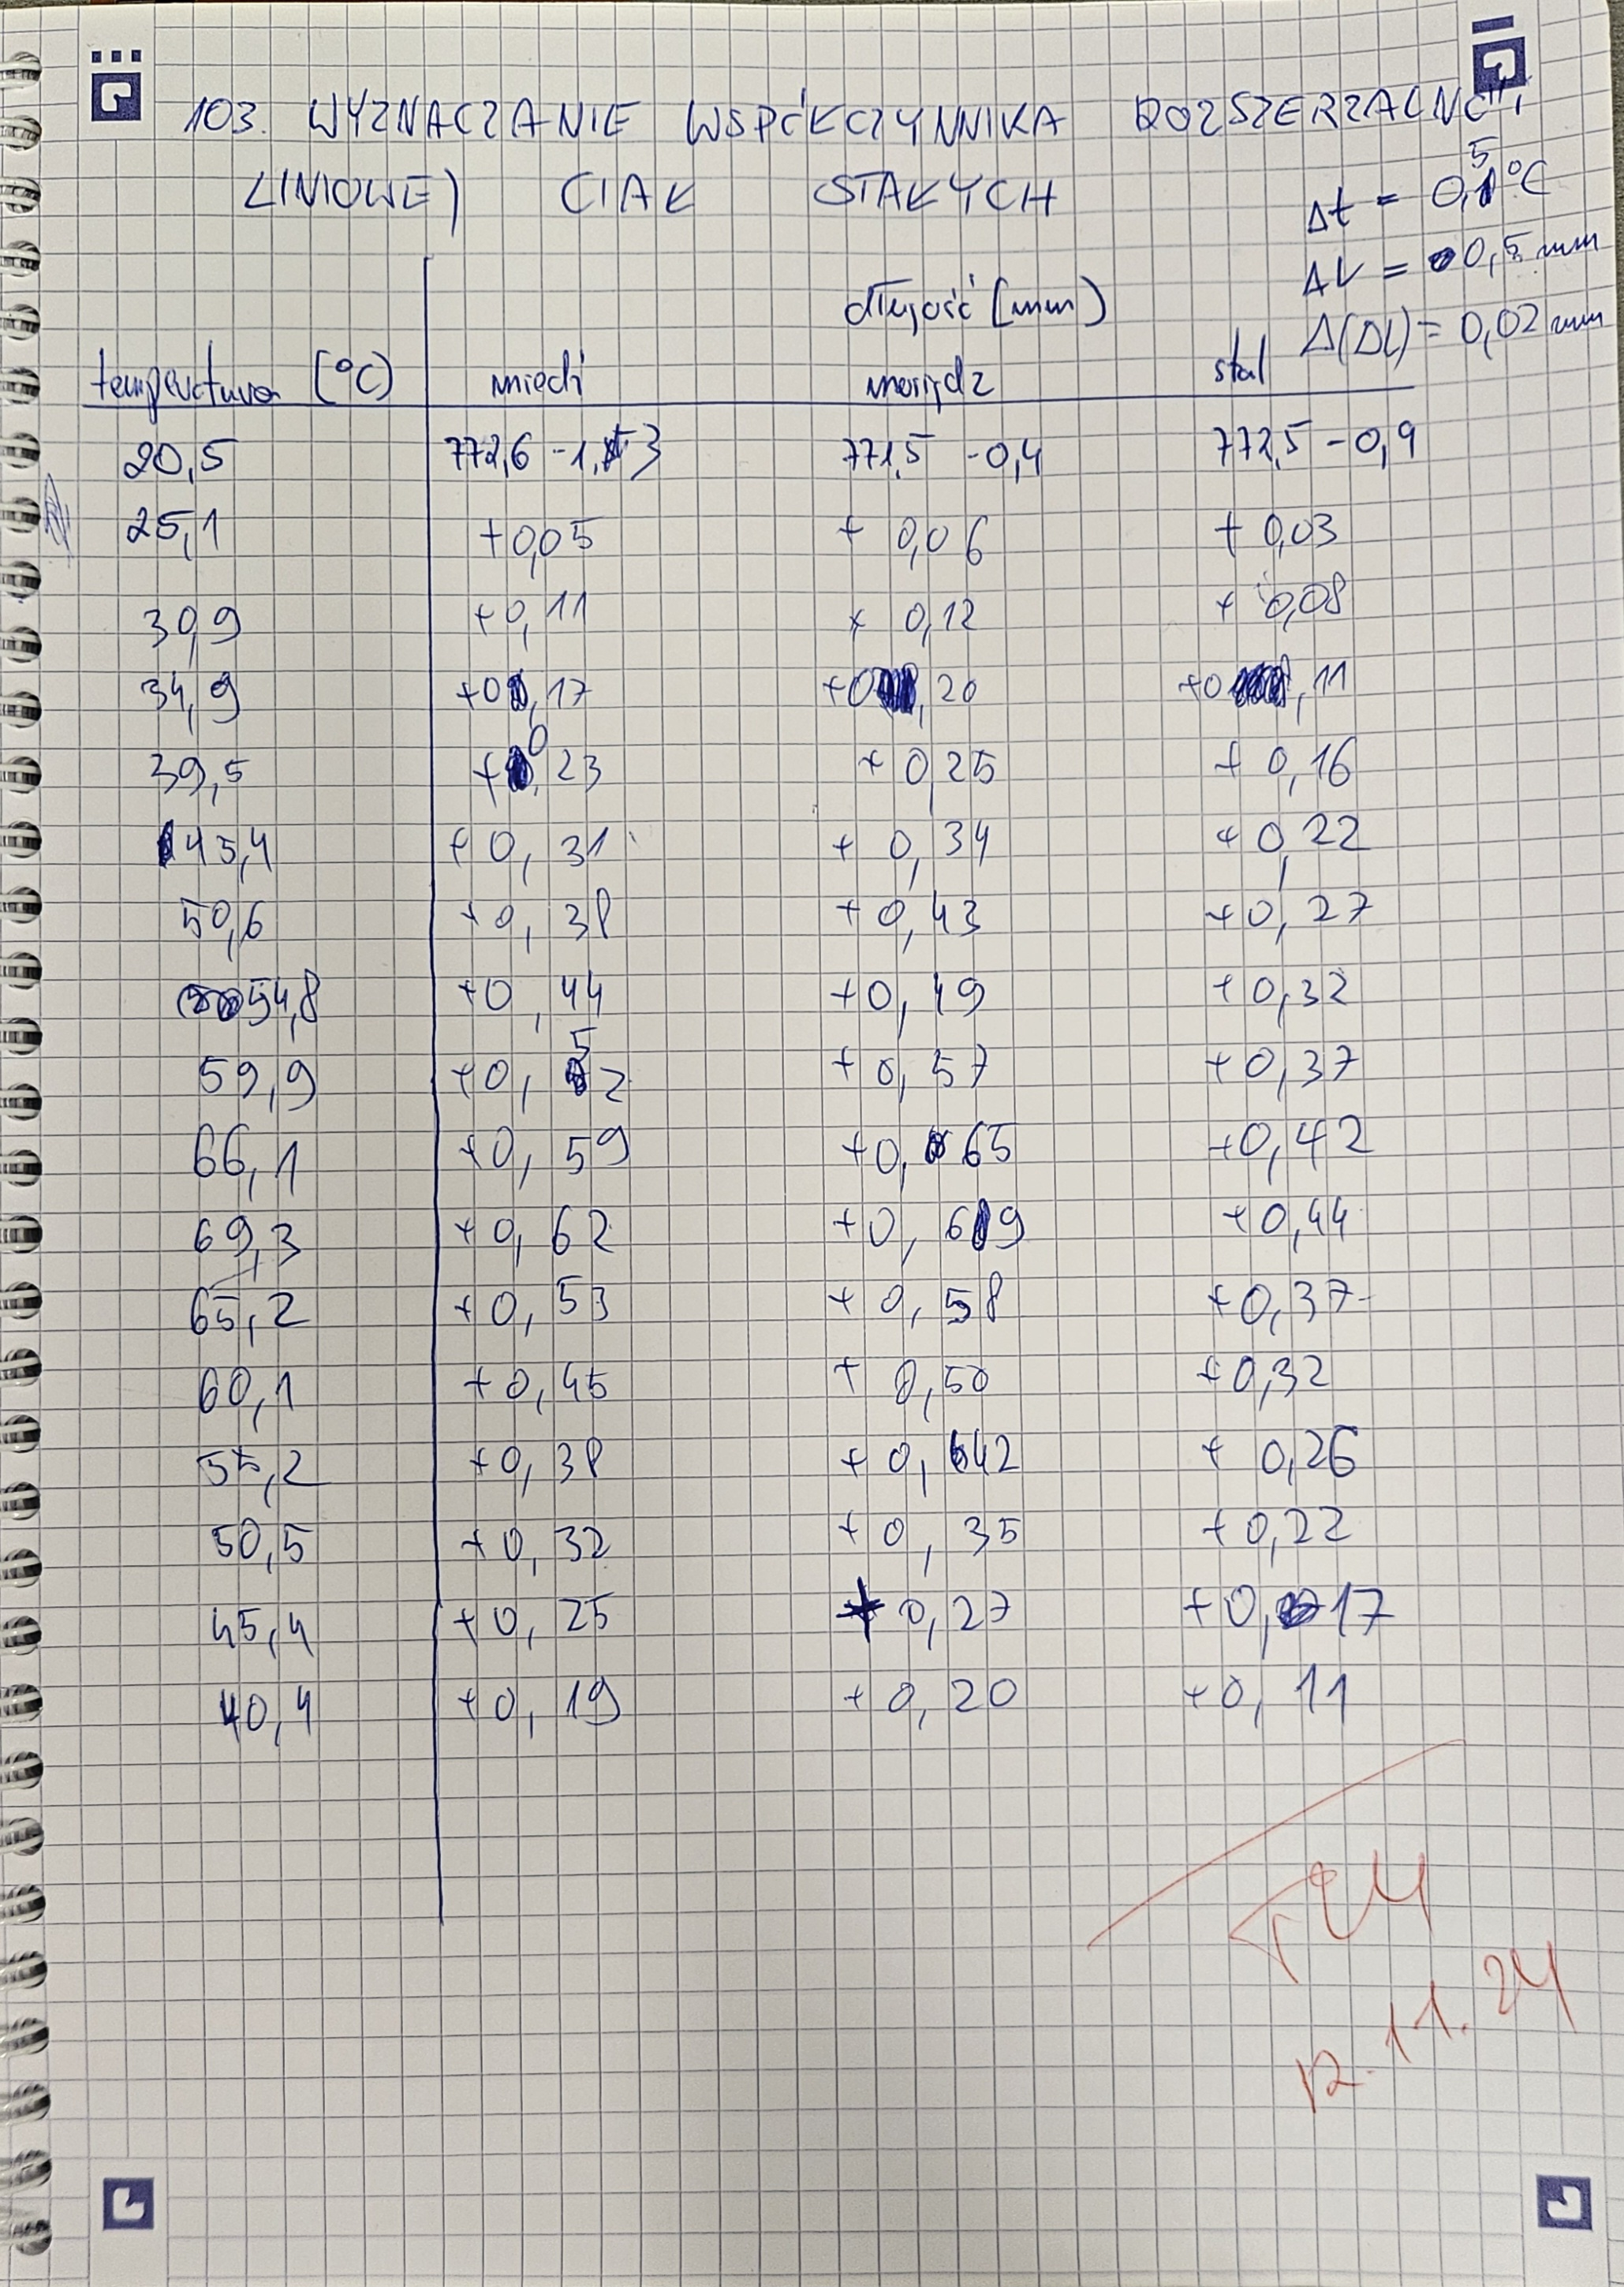
\includegraphics[scale=0.22]{images/pomiary.jpg}
\end{center}
% subsection Zdjecie wynikow pomiarow (end)

\pagebreak
\section{Opracowanie wyników}\label{sec:opracowanie_wynikow} % (fold)

\subsection{Wykres}\label{sub:wykres} % (fold)
\begin{center}
	\begin{tikzpicture}
		\node (img) {
			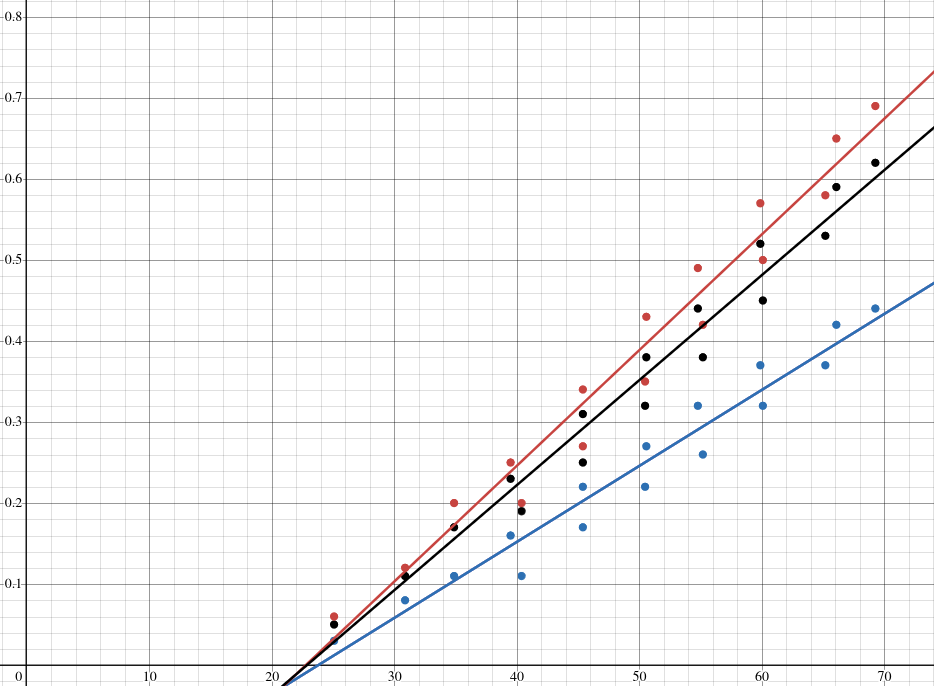
\includegraphics[scale=0.5]{images/wykres.png}
		};
		\draw[->, thick] (-8,-5.7) -- (8.5,-5.7) node[anchor=south east] {temperatura [$^{\circ} C$]};
		\draw[->, thick] (-7.8,-6) -- (-7.8,6.4) node[anchor=north west] {wydłużenie [mm]};
	\end{tikzpicture}
\end{center}
Kolory:
\begin{itemize}
	\item Czerwony - mosiądz
	\item Czarny - miedź
	\item Niebieski - stal
\end{itemize}
% subsection Wykres (end)

\subsection{Obliczenia}\label{sub:obliczenia} % (fold)
W celu wyznaczenia współczynnika rozszerzalności z danych pomiarowych zapiszemy równanie \eqref{eq:alpha2} w postaci:
\begin{equation}
	\Delta l = \alpha_{sr} l_0 T - \alpha_{sr} l_0 T_0
\end{equation}
Równanie to oznacza, że wydłużenie jest linową funkcją temperatury i że współczynnik nachylenia prostej
$a = \alpha_{sr}l_0$ . Więc współczynnik rozszerzalności wyznaczymy ze wzoru:
\begin{equation}
	\alpha = \frac{a}{l_0}
\end{equation}

% subsection Obliczenia (end)

\subsubsection{Miedź}\label{sub:miedz} % (fold)
Równanie prostej:
\[
	y = 0,0129592x - 0,296283
\]


% subsection Miedz (end)

\subsubsection{Mosiądz}\label{sub:mosiadz} % (fold)
Równanie prostej:
\[
	y = 0,0142768x - 0,325362
\]
% subsection Mosiadz (end)

\subsubsection{Stal}\label{sub:stal} % (fold)
Równanie prostej:
\[
	y = 0,00937915x - 0,223155
\]
% subsection Stal (end)

\subsection{Wyniki}\label{sub:wyniki} % (fold)

% subsection Wyniki (end)

\subsection{Wnioski}\label{sub:wnioski} % (fold)

% subsection Wnioski (end)

\end{document}

